Volg de instructies op \url{https://learn.microsoft.com/en-us/windows/python/scripting} om Python te installeren. Alleen het kopje \textquote{Install Python}. Je installeert nu de Python-interpreter.

Als Python ge\"installeerd is kan je via de zoekbalk Python opzoeken en opstarten, zoals je kan zien in \ref{fig:pythonint}

\begin{figure}[H]
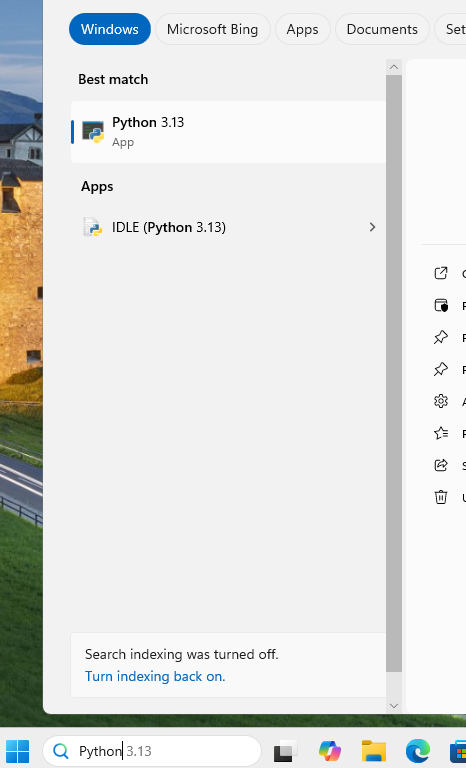
\includegraphics[width=0.9\textwidth]{Screenshot-Python-Start-Selection.png}
        \caption{Zoek en start Python}
        \label{fig:pythonint}
\end{figure}

Om de Python-interpreter af te sluiten type je \texttt{exit()}. Denk om de haakjes aan het einde.
